\documentclass[a4paper,12pt,oneside]{book}
\usepackage[utf8]{inputenc}
\title{}
\author{Rachel Morris}
\date{\today}

\usepackage{rachwidgets}
\usepackage{fancyhdr}
\usepackage{lastpage}
\usepackage{boxedminipage}
\usepackage{fancyvrb}

\newcommand{\laClass}{CS 250\ }
\newcommand{\laSemester}{Fall 2017\ }
\newcommand{\laLab}{Lab 13: Trees\ }
\newcounter{question}

\pagestyle{fancy}
\fancyhf{}
\lhead{\laClass}
\chead{\laSemester}
\rhead{\laLab}
\rfoot{\thepage\ of \pageref{LastPage}}
\lfoot{By Rachel Morris, \footnotesize last updated \today}

\renewcommand{\headrulewidth}{2pt}
\renewcommand{\footrulewidth}{1pt}

%\toggletrue{answerkey}
\togglefalse{answerkey}

%
%
%       MAKE SURE TO ADD TEXT TO SPECIFY THE DIFFERENCE BETWEEN A *BINARY TREE* AND A *BINARY SEARCH TREE*!
%
%

\begin{document}

    \chapter*{\laLab} \stepcounter{chapter}

        \section{Information}
            \paragraph{ Topics: } Trees
            \paragraph{ Turn in: } This is another on-paper ``lab". Turn in a text file, PDF file, scanned or photographed images.
            
% ----------------------------------------------------------------------
% ----------------------------------------------------------------------
% ----------------------------------------------------------------------

    \hrulefill

    \section{About: Efficiency}

    Every data structure has trade-offs. For example,
    it is faster to access items at some position in an array
    than it is to do so in a linked list. However, if the array is
    unsorted, there is not a good efficient way to search the array
    to find some specific data.
    If we were to build a sorted array, we would have to
    decide \textit{when} to do the sorting...

    \begin{itemize}
        \item   During Insert - Locate the proper place for the new data
        \item   After Insert - Insert to the end, then re-sort the array
    \end{itemize}

    Either way, the act of inserting data into the array will slow
    down the process, since we would need to either shift $n$ items over
    to make room for the new item, or perform a sorting algorithm;
    neither way is as efficient as simply putting data in the array at the
    end, but it might make \textit{access time} more efficient.

    When selecting a data structure to use, part of what we need to consider
    is what we're designing and how the data structure will be used -
    will we do a lot of inserts? Will we do a lot of accesses?
    If we're inserting data often but not reading that data very much,
    a structure like a Linked List or Unsorted Array might be fine,
    with $O(1)$ time for the ``push" function. If we don't do
    insertions very often, but need to read the data frequently,
    it would be better to keep our data sorted.

    \begin{center}
        \begin{tikzpicture}
            \filldraw (0,5) circle (1pt) node[above] {D};
            \filldraw (-2,4) circle (1pt) node[above] {B};
            \filldraw (2,4) circle (1pt) node[above] {F};
            \filldraw (-3,3) circle (1pt) node[below] {A};
            \filldraw (-1,3) circle (1pt) node[below] {C};
            \filldraw (1,3) circle (1pt) node[below] {E};
            \filldraw (3,3) circle (1pt) node[above] {H};
            \filldraw (2,2) circle (1pt) node[below] {G};            
            \filldraw (4,2) circle (1pt) node[below] {I};
            
            \draw (0, 5) -- (-2, 4) -- (-3, 3);
            \draw (-2, 4) -- (-1, 3);
            \draw (0, 5) -- (2, 4) -- (1, 3);
            \draw (2, 4) -- (3, 3);
            \draw (3, 3) -- (2, 2);
            \draw (3, 3) -- (4, 2);
            
            \draw[->] (0,0) -- (-1,0) node[left] {Smaller};
            \draw[->] (0,0) -- (1,0) node[right] {Larger};

        \end{tikzpicture}
    \end{center}

    Trees, especially Binary Search Trees (which we will talk about on its own),
    are a type of structure where we can make a compromise. Specifically
    for a \textbf{Binary Search Tree}, insert and access are both $O(log\ n)$
    on average, because as we traverse through the tree, each step we're
    removing \textit{half} of the search space.

    ~\\
    We will return to Binary Search Trees later, but for now let's go
    over the terminology associated with Trees.

    \section{Intro to Trees}

    \paragraph{Tree:} A collection of \textbf{Nodes (or vertices)} and \textbf{Edges}.

    \paragraph{Edge:} A path that connects two Nodes together. If we have $N$ nodes,
        then there are $N-1$ edges.

    \paragraph{Nodes:} A vertex in the tree, usually associated with some data.

    \subparagraph{Root Node:} The source Node of the tree; it has no parents.
    Each Tree has one Root Node, usually drawn at the top. All
    other Nodes descend from the Root Node.
    
    \subparagraph{Leaf Node:} A Node with no children.
    
    \subparagraph{Node Family:} We use family terminology to talk about
        how Nodes are related to each other.

        \begin{itemize}
            \item   \textbf{Parent node:} Given some Node $n$, $n$'s parent
                is the Node immediately above $n$, in the path between $n$
                and the root node. Each Node can have only 0 or 1 parent.

            \item   \textbf{Ancestor node:} Given some Node $n$, an Ancestor
                of $n$ is any Node along the path from $n$ to the root node.

            \item   \textbf{Child node:} Given some Node $n$, $n$'s child
                is a Node that comes immediately below it in the tree.
                Node $n$ lies in the path from its child to the root node.
                Each Node can have 0 or more children. With a Binary Search Tree,
                a Node can have 0, 1, or 2 children.

            \item   \textbf{Descendant node:} Given some Node $n$, a
                Descendant is a Node that comes below it in the tree, where
                the Node $n$ lies in the path from that descendant to the root node.

            \item   \textbf{Sibling node:} Given some Node $n$, a Sibling
                of $n$ is another Node where $n$ and that Sibling share the same
                Parent node.
        \end{itemize}

        \hrulefill

        % -------------------------------------------------------------%
        % - QUESTION --------------------------------------------------%
        % -------------------------------------------------------------%
        \stepcounter{question}
        \begin{question}{\thequestion}{4}

            For the given tree:
            
            \begin{center}
                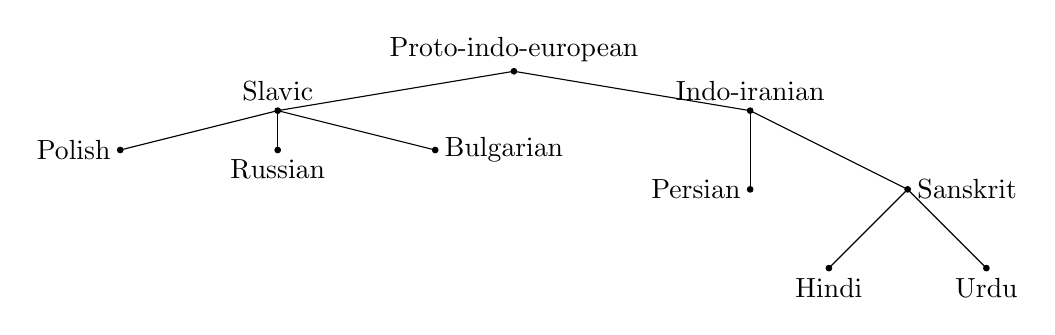
\begin{tikzpicture}
                    \filldraw (0,5) circle (1pt) node[above] {Proto-indo-european};
                    
                    \filldraw (-3,4.5) circle (1pt) node[above] {Slavic};
                    \filldraw (3,4.5) circle (1pt) node[above] {\tab Indo-iranian};
                    \draw (0,5) -- (-3,4.5);
                    \draw (0,5) -- (3,4.5);
                    
                    \filldraw (-5,4) circle (1pt) node[left] {Polish};
                    \filldraw (-3,4) circle (1pt) node[below] {Russian};
                    \filldraw (-1,4) circle (1pt) node[right] {Bulgarian};
                    \draw (-3,4.5) -- (-5,4);
                    \draw (-3,4.5) -- (-3,4);
                    \draw (-3,4.5) -- (-1,4);
                    
                    \filldraw (3,3.5) circle (1pt) node[left] {Persian};
                    \filldraw (5,3.5) circle (1pt) node[right] {Sanskrit};
                    \draw (3,4.5) -- (3,3.5);
                    \draw (3,4.5) -- (5,3.5);
                    
                    \filldraw (4,2.5) circle (1pt) node[below] {Hindi};            
                    \filldraw (6,2.5) circle (1pt) node[below] {Urdu};
                    \draw (5,3.5) -- (4,2.5);
                    \draw (5,3.5) -- (6,2.5);
                    
                \end{tikzpicture}
            \end{center}

            \begin{itemize}
                \item[a.]   What are all the (listed) ancestors of $Russian$?
                    \solution{ Slavic, Proto-indo-european }{ \vspace{0.5cm} }
                
                \item[b.]   What are all the (listed) descendants of $Indo-iranian$?
                    \solution{ Persian, Sanskrit, Hindi, Urdu }{ \vspace{0.5cm} }
                
                \item[c.]   What are all the (listed) siblings of $Polish$?
                    \solution{ Russian and Bulgarian }{ \vspace{0.5cm} }
                
                \item[d.]   What are all the (listed) leaves of the tree?
                    \solution{ Polish, Russian, Bulgarian, Persian, Hindi, Urdu }{ \vspace{0.5cm} }
            \end{itemize}
            
        \end{question}

    \newpage

        \paragraph{Path:} A path between two nodes, $n_{a}$ and $n_{b}$,
            is a series of connecting edges between these two nodes.

            \subparagraph{Path Length:} The Length of a Path is the
                amount of edges in the path.

        \paragraph{Node Depth:} Given any node $n$, the Depth of $n$ is
            the \textit{length} of the path between $n$ and the root.
        
        \paragraph{Node Height:} Given any node $n$, the Height of $n$ is
            the longest path from $n$ to a leaf. Leaves have a height of 0.

        \hrulefill
        
        % -------------------------------------------------------------%
        % - QUESTION --------------------------------------------------%
        % -------------------------------------------------------------%
        \stepcounter{question}
        \begin{question}{\thequestion}{4}

            For the given tree:
            
            \begin{center}
                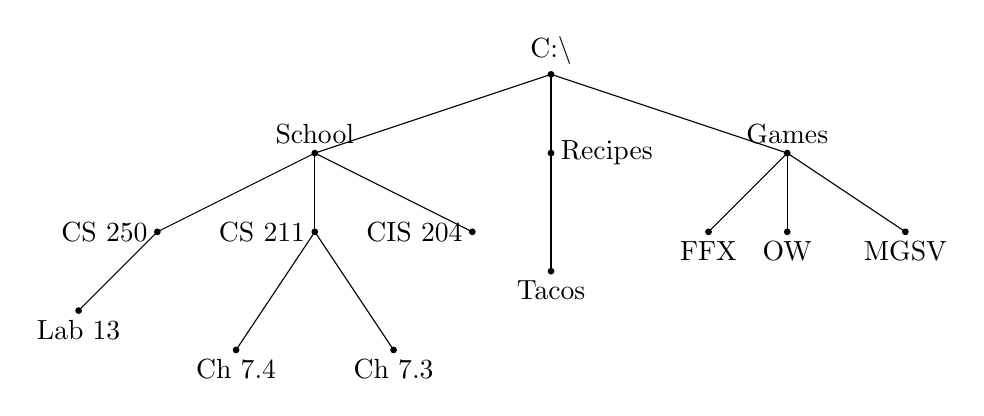
\begin{tikzpicture}
                    \filldraw (0,5) circle (1pt) node[above] { C:$\backslash$ };
                    
                    \filldraw (-3,4) circle (1pt) node[above] {School};
                    \filldraw (0,4) circle (1pt) node[right] {Recipes};
                    \filldraw (3,4) circle (1pt) node[above] {Games};                    
                    \draw (0,5) -- (-3,4);
                    \draw (0,5) -- (-0,4);
                    \draw (0,5) -- (3,4);

                    \filldraw(-5, 3) circle (1pt) node[left] {CS 250};
                    \filldraw(-3, 3) circle (1pt) node[left] {CS 211};
                    \filldraw(-1, 3) circle (1pt) node[left] {CIS 204};
                    \draw(-3,4) -- (-5, 3);
                    \draw(-3,4) -- (-3, 3);
                    \draw(-3,4) -- (-1, 3);

                    \filldraw(-6,2) circle (1pt) node[below] {Lab 13};
                    \draw(-5,3) -- (-6,2);
                    
                    \filldraw(-2,1.5) circle (1pt) node[below] {Ch 7.3};
                    \filldraw(-4,1.5) circle (1pt) node[below] {Ch 7.4};
                    \draw(-3,3) -- (-2,1.5);
                    \draw(-3,3) -- (-4,1.5);

                    \filldraw(0, 2.5) circle (1pt) node[below] {Tacos};
                    \draw(0,4) -- (0,2.5);

                    \filldraw(2,3) circle (1pt) node[below] {FFX};
                    \filldraw(3,3) circle (1pt) node[below] {OW};
                    \filldraw(4.5,3) circle (1pt) node[below] {MGSV};
                    \draw(3,4) -- (2,3);
                    \draw(3,4) -- (3,3);
                    \draw(3,4) -- (4.5,3);
                    
                \end{tikzpicture}
            \end{center}

            \begin{itemize}
                \item[a.]   Write out all the Nodes in the path from \textit{Lab 13} to \textit{C:$\backslash$}.
                    \solution{ Lab 13 $\to$ CS 250 $\to$ School $\to$ C:$\backslash$ }{ \vspace{0.5cm} }

                \item[b.]   What is the length of the path from \textit{Lab 13} to \textit{C:$\backslash$}?
                    \solution{ 3 }{ \fitb }

                \item[c.]   Find the Depths and Heights for the following:
                    \begin{center}
                        \begin{tabular}{c | c | c}
                            Node & Depth & Height \\ \hline
                            Lab 13
                                & \solution{3}{}
                                & \solution{0}{}
                            \\ \hline
                            Ch 7.3
                                & \solution{3}{}
                                & \solution{0}{}
                            \\ \hline
                            Tacos
                                & \solution{2}{}
                                & \solution{0}{}
                            \\ \hline
                            MGSV
                                & \solution{2}{}
                                & \solution{0}{}
                            \\ \hline
                            CS 211
                                & \solution{2}{}
                                & \solution{1}{}
                            \\ \hline
                            School
                                & \solution{1}{}
                                & \solution{2}{}
                        \end{tabular}
                    \end{center}
                

            \end{itemize}
            
        \end{question}

    \newpage

    \subsection{Traversals}
    
        \begin{center}
            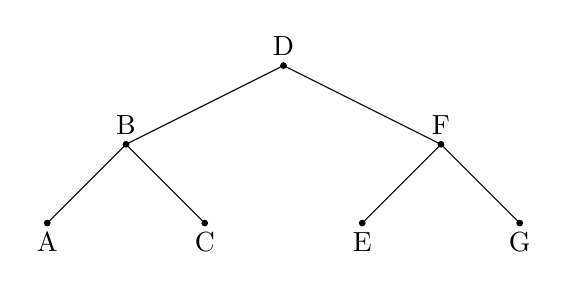
\begin{tikzpicture}
                \filldraw (0,5) circle (1pt) node[above] {D};
                \filldraw (-2,4) circle (1pt) node[above] {B};
                \filldraw (2,4) circle (1pt) node[above] {F};
                \filldraw (-3,3) circle (1pt) node[below] {A};
                \filldraw (-1,3) circle (1pt) node[below] {C};
                \filldraw (1,3) circle (1pt) node[below] {E};
                \filldraw (3,3) circle (1pt) node[below] {G};
                
                \draw (0, 5) -- (-2, 4) -- (-3, 3);
                \draw (-2, 4) -- (-1, 3);
                \draw (0, 5) -- (2, 4) -- (1, 3);
                \draw (2, 4) -- (3, 3);
            \end{tikzpicture}
        \end{center}

        Since a Tree is not a linear structure, what order do you
        display its contents? There are three main methods you
        will see for traversing through a tree. Each of these
        are recursive, beginning at the root node.
        Once the end of a path is reached (by hitting a leaf),
        the recursion causes it to step back upwards through the tree.

        \paragraph{Pre-order traversal}
            Begin at the Root $r$ node of some Tree/Subtree...
            
            \begin{enumerate}
                \item   Process $r$
                \item   Traverse left, if available
                \item   Traverse right, if available
            \end{enumerate}

            With the above tree, we process nodes as such: \\ \tab
            \texttt{ D - B - A - C - F - E - G }

        \paragraph{In-order traversal}
            Begin at the Root $r$ node of some Tree/Subtree...
            
            \begin{enumerate}
                \item   Traverse left, if available
                \item   Process $r$
                \item   Traverse right, if available
            \end{enumerate}

            With the above tree, we process nodes as such: \\ \tab
            \texttt{ A - B - C - D - E - F - G }

        \paragraph{Post-order traversal}
            Begin at the Root $r$ node of some Tree/Subtree...
            
            \begin{enumerate}
                \item   Traverse left, if available
                \item   Traverse right, if available
                \item   Process $r$
            \end{enumerate}

            With the above tree, we process nodes as such: \\ \tab
            \texttt{ A - C - B - E - G - F - D }

        \newpage

        \begin{center}\textbf{Step-by-step pre-order illustration:}\end{center}

        \begin{tabular}{p{5cm} p{1cm} p{5cm}}

            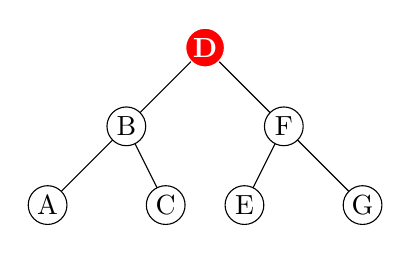
\begin{tikzpicture}
                \draw (0, 5) -- (-1,4);
                \draw (0, 5) -- (1,4);
                \draw (-1,4) -- (-2,3);
                \draw (-1,4) -- (-0.5,3);
                \draw (1,4) -- (2,3);
                \draw (1,4) -- (0.5,3);
            
                \draw[white,fill=red]
                    (0,5)  circle (7pt) node {\textbf{D}};
                \draw[fill=white] 
                    (-1,4) circle (7pt) node {B};
                \draw[fill=white] 
                    (1,4)  circle (7pt) node {F};
                \draw[fill=white] 
                    (-2,3) circle (7pt) node {A};
                \draw[fill=white] 
                    (-0.5,3) circle (7pt) node {C};
                \draw[fill=white] 
                    (0.5,3)  circle (7pt) node {E};
                \draw[fill=white] 
                    (2,3)  circle (7pt) node {G};
            \end{tikzpicture}
            & &
            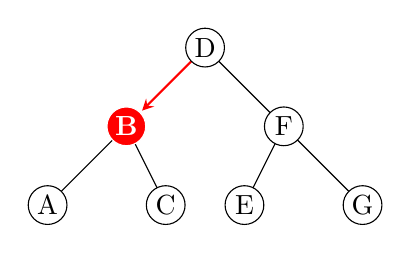
\begin{tikzpicture}[arrow/.style = {thick,-stealth}]
                \draw[red,arrow] (0, 5) -- (-0.8,4.2);
                \draw (0, 5) -- (1,4);
                \draw (-1,4) -- (-2,3);
                \draw (-1,4) -- (-0.5,3);
                \draw (1,4) -- (2,3);
                \draw (1,4) -- (0.5,3);
            
                \draw[fill=white] 
                    (0,5)  circle (7pt) node {D};
                \draw[white,fill=red] 
                    (-1,4) circle (7pt) node {\textbf{B}};
                \draw[fill=white] 
                    (1,4)  circle (7pt) node {F};
                \draw[fill=white] 
                    (-2,3) circle (7pt) node {A};
                \draw[fill=white] 
                    (-0.5,3) circle (7pt) node {C};
                \draw[fill=white] 
                    (0.5,3)  circle (7pt) node {E};
                \draw[fill=white] 
                    (2,3)  circle (7pt) node {G};
            \end{tikzpicture}
            \\ \footnotesize 
            1. Begin at D. Process ``D" then go left. 
            & & \footnotesize 
            2. Process ``B" then go left.
            \\ \footnotesize 
            Output: \texttt{D} 
            & & \footnotesize 
            Output: \texttt{D B} 
            \\ \\ \\
            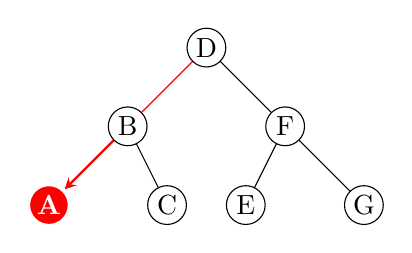
\begin{tikzpicture}[arrow/.style = {thick,-stealth}]
                \draw[red] (0, 5) -- (-1,4);
                \draw (0, 5) -- (1,4);
                \draw[arrow,red] (-1,4) -- (-1.8,3.2);
                \draw (-1,4) -- (-0.5,3);
                \draw (1,4) -- (2,3);
                \draw (1,4) -- (0.5,3);
            
                \draw[fill=white] 
                    (0,5)  circle (7pt) node {D};
                \draw[fill=white] 
                    (-1,4) circle (7pt) node {B};
                \draw[fill=white] 
                    (1,4)  circle (7pt) node {F};
                \draw[white,fill=red] 
                    (-2,3) circle (7pt) node {\textbf{A}};
                \draw[fill=white] 
                    (-0.5,3) circle (7pt) node {C};
                \draw[fill=white] 
                    (0.5,3)  circle (7pt) node {E};
                \draw[fill=white] 
                    (2,3)  circle (7pt) node {G};
            \end{tikzpicture}
            & &
            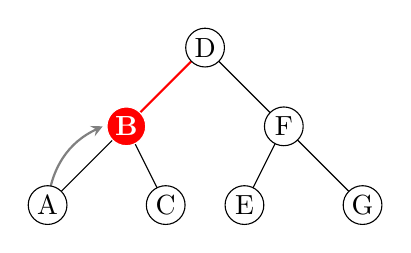
\begin{tikzpicture}[arrow/.style = {thick,-stealth}]
                \draw[red,arrow] (0, 5) -- (-1,4);
                \draw (0, 5) -- (1,4);
                \draw (-1,4) -- (-2,3);
                \draw (-1,4) -- (-0.5,3);
                \draw (1,4) -- (2,3);
                \draw (1,4) -- (0.5,3);
                
                \draw[arrow,gray] (-2,3) to[bend left] (-1.3,4);
            
                \draw[fill=white] 
                    (0,5)  circle (7pt) node {D};
                \draw[white,fill=red] 
                    (-1,4) circle (7pt) node {\textbf{B}};
                \draw[fill=white] 
                    (1,4)  circle (7pt) node {F};
                \draw[fill=white] 
                    (-2,3) circle (7pt) node {A};
                \draw[fill=white] 
                    (-0.5,3) circle (7pt) node {C};
                \draw[fill=white] 
                    (0.5,3)  circle (7pt) node {E};
                \draw[fill=white] 
                    (2,3)  circle (7pt) node {G};
            \end{tikzpicture}
            \\ \footnotesize 
            3. Process ``A"; no more children, return (back to B).
            & & \footnotesize 
            4. Go to right child.
            \\ \footnotesize 
            Output: \texttt{D B A} 
            & & \footnotesize 
            Output: \texttt{D B A}
            \\ \\ \\
            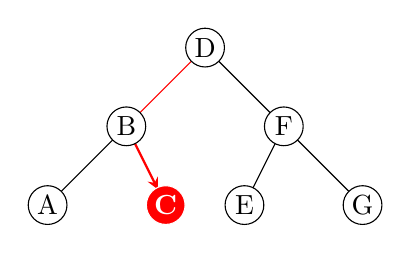
\begin{tikzpicture}[arrow/.style = {thick,-stealth}]
                \draw[red] (0, 5) -- (-1,4);
                \draw (0, 5) -- (1,4);
                \draw (-1,4) -- (-2,3);
                \draw[red,arrow] (-1,4) -- (-0.6,3.2);
                \draw (1,4) -- (2,3);
                \draw (1,4) -- (0.5,3);
            
                \draw[fill=white] 
                    (0,5)  circle (7pt) node {D};
                \draw[fill=white] 
                    (-1,4) circle (7pt) node {B};
                \draw[fill=white] 
                    (1,4)  circle (7pt) node {F};
                \draw[fill=white] 
                    (-2,3) circle (7pt) node {A};
                \draw[white,fill=red] 
                    (-0.5,3) circle (7pt) node {\textbf{C}};
                \draw[fill=white] 
                    (0.5,3)  circle (7pt) node {E};
                \draw[fill=white] 
                    (2,3)  circle (7pt) node {G};
            \end{tikzpicture}
            & &
            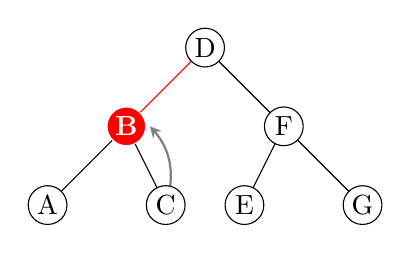
\begin{tikzpicture}[arrow/.style = {thick,-stealth}]
                \draw[red] (0, 5) -- (-1,4);
                \draw (0, 5) -- (1,4);
                \draw (-1,4) -- (-2,3);
                \draw (-1,4) -- (-0.5,3);
                \draw (1,4) -- (2,3);
                \draw (1,4) -- (0.5,3);
                \draw[arrow,gray] (-0.5,3) to[bend right] (-0.7,4);
            
                \draw[fill=white] 
                    (0,5)  circle (7pt) node {D};
                \draw[white,fill=red] 
                    (-1,4) circle (7pt) node {\textbf{B}};
                \draw[fill=white] 
                    (1,4)  circle (7pt) node {F};
                \draw[fill=white] 
                    (-2,3) circle (7pt) node {A};
                \draw[fill=white] 
                    (-0.5,3) circle (7pt) node {C};
                \draw[fill=white] 
                    (0.5,3)  circle (7pt) node {E};
                \draw[fill=white] 
                    (2,3)  circle (7pt) node {G};
            \end{tikzpicture}
            \\ \footnotesize 
            5. Process ``C"; no more children, return (back to B).
            & & \footnotesize 
            6. Done with left and right subtrees, return (back to D).
            \\ \footnotesize 
            Output: \texttt{D B A C} 
            & & \footnotesize 
            Output: \texttt{D B A C}
            \\ \\ \\
            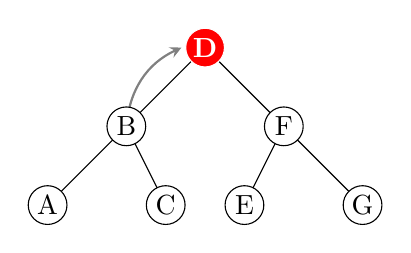
\begin{tikzpicture}[arrow/.style = {thick,-stealth}]
                \draw (0, 5) -- (-1,4);
                \draw (0, 5) -- (1,4);
                \draw (-1,4) -- (-2,3);
                \draw (-1,4) -- (-0.5,3);
                \draw (1,4) -- (2,3);
                \draw (1,4) -- (0.5,3);
                \draw[arrow,gray] (-1,4) to[bend left] (-0.3,5);
            
                \draw[white,fill=red] 
                    (0,5)  circle (7pt) node {\textbf{D}};
                \draw[fill=white] 
                    (-1,4) circle (7pt) node {B};
                \draw[fill=white] 
                    (1,4)  circle (7pt) node {F};
                \draw[fill=white] 
                    (-2,3) circle (7pt) node {A};
                \draw[fill=white] 
                    (-0.5,3) circle (7pt) node {C};
                \draw[fill=white] 
                    (0.5,3)  circle (7pt) node {E};
                \draw[fill=white] 
                    (2,3)  circle (7pt) node {G};
            \end{tikzpicture}
            & &
            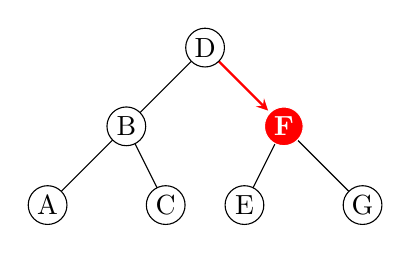
\begin{tikzpicture}[arrow/.style = {thick,-stealth}]
                \draw (0, 5) -- (-1,4);
                \draw[red,arrow] (0, 5) -- (0.8,4.2);
                \draw (-1,4) -- (-2,3);
                \draw (-1,4) -- (-0.5,3);
                \draw (1,4) -- (2,3);
                \draw (1,4) -- (0.5,3);
            
                \draw[fill=white] 
                    (0,5)  circle (7pt) node {D};
                \draw[fill=white] 
                    (-1,4) circle (7pt) node {B};
                \draw[white,fill=red] 
                    (1,4)  circle (7pt) node {\textbf{F}};
                \draw[fill=white] 
                    (-2,3) circle (7pt) node {A};
                \draw[fill=white] 
                    (-0.5,3) circle (7pt) node {C};
                \draw[fill=white] 
                    (0.5,3)  circle (7pt) node {E};
                \draw[fill=white] 
                    (2,3)  circle (7pt) node {G};
            \end{tikzpicture}
            \\ \footnotesize 
            5. Go to right child.
            & & \footnotesize 
            6. Process ``F" then go left.
            \\ \footnotesize 
            Output: \texttt{D B A C} 
            & & \footnotesize 
            Output: \texttt{D B A C F}
            \\ \\ \\
            
        \end{tabular}

        \newpage

        
        \begin{tabular}{p{5cm} p{1cm} p{5cm}}
            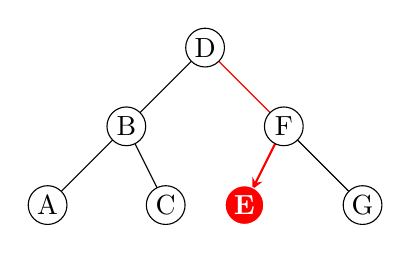
\begin{tikzpicture}[arrow/.style = {thick,-stealth}]
                \draw (0, 5) -- (-1,4);
                \draw[red] (0, 5) -- (1,4);
                \draw (-1,4) -- (-2,3);
                \draw (-1,4) -- (-0.5,3);
                \draw (1,4) -- (2,3);
                \draw[red,arrow] (1,4) -- (0.6,3.2);
            
                \draw[fill=white] 
                    (0,5)  circle (7pt) node {D};
                \draw[fill=white] 
                    (-1,4) circle (7pt) node {B};
                \draw[fill=white] 
                    (1,4)  circle (7pt) node {F};
                \draw[fill=white] 
                    (-2,3) circle (7pt) node {A};
                \draw[fill=white] 
                    (-0.5,3) circle (7pt) node {C};
                \draw[white,fill=red] 
                    (0.5,3)  circle (7pt) node {\textbf{E}};
                \draw[fill=white] 
                    (2,3)  circle (7pt) node {G};
            \end{tikzpicture}
            & &
            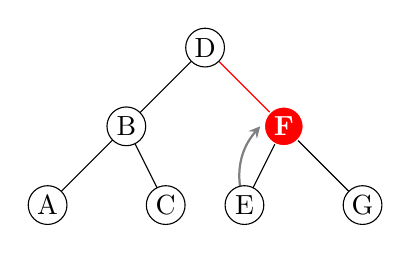
\begin{tikzpicture}[arrow/.style = {thick,-stealth}]
                \draw (0, 5) -- (-1,4);
                \draw[red] (0, 5) -- (1,4);
                \draw (-1,4) -- (-2,3);
                \draw (-1,4) -- (-0.5,3);
                \draw (1,4) -- (2,3);
                \draw (1,4) -- (0.5,3);
                \draw[arrow,gray] (0.5,3) to[bend left] (0.7,4);
            
                \draw[fill=white] 
                    (0,5)  circle (7pt) node {D};
                \draw[fill=white] 
                    (-1,4) circle (7pt) node {B};
                \draw[white,fill=red] 
                    (1,4)  circle (7pt) node {\textbf{F}};
                \draw[fill=white] 
                    (-2,3) circle (7pt) node {A};
                \draw[fill=white] 
                    (-0.5,3) circle (7pt) node {C};
                \draw[fill=white] 
                    (0.5,3)  circle (7pt) node {E};
                \draw[fill=white] 
                    (2,3)  circle (7pt) node {G};
            \end{tikzpicture}
            \\  \footnotesize 
            7. Process ``E" then return (back to F).
            & &   \footnotesize 
            8. Go to right child.
            \\  \footnotesize 
            Output: \texttt{D B A C F E}
            & &  \footnotesize 
            Output: \texttt{D B A C F E}
            \\ \\ \\
            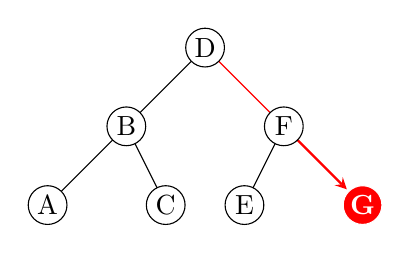
\begin{tikzpicture}[arrow/.style = {thick,-stealth}]
                \draw (0, 5) -- (-1,4);
                \draw[red] (0, 5) -- (1,4);
                \draw (-1,4) -- (-2,3);
                \draw (-1,4) -- (-0.5,3);
                \draw[red,arrow] (1,4) -- (1.8,3.2);
                \draw (1,4) -- (0.5,3);
            
                \draw[fill=white] 
                    (0,5)  circle (7pt) node {D};
                \draw[fill=white] 
                    (-1,4) circle (7pt) node {B};
                \draw[fill=white] 
                    (1,4)  circle (7pt) node {F};
                \draw[fill=white] 
                    (-2,3) circle (7pt) node {A};
                \draw[fill=white] 
                    (-0.5,3) circle (7pt) node {C};
                \draw[fill=white] 
                    (0.5,3)  circle (7pt) node {E};
                \draw[white,fill=red] 
                    (2,3)  circle (7pt) node {\textbf{G}};
            \end{tikzpicture}
            & &
            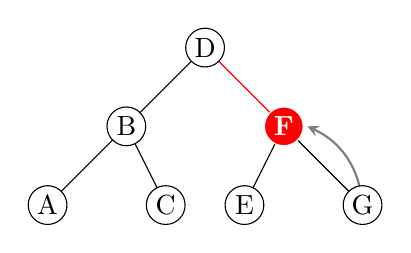
\begin{tikzpicture}[arrow/.style = {thick,-stealth}]
                \draw (0, 5) -- (-1,4);
                \draw[red] (0, 5) -- (1,4);
                \draw (-1,4) -- (-2,3);
                \draw (-1,4) -- (-0.5,3);
                \draw (1,4) -- (2,3);
                \draw (1,4) -- (0.5,3);
                \draw[arrow,gray] (2,3) to[bend right] (1.3,4);
            
                \draw[fill=white] 
                    (0,5)  circle (7pt) node {D};
                \draw[fill=white] 
                    (-1,4) circle (7pt) node {B};
                \draw[white,fill=red] 
                    (1,4)  circle (7pt) node {\textbf{F}};
                \draw[fill=white] 
                    (-2,3) circle (7pt) node {A};
                \draw[fill=white] 
                    (-0.5,3) circle (7pt) node {C};
                \draw[fill=white] 
                    (0.5,3)  circle (7pt) node {E};
                \draw[fill=white] 
                    (2,3)  circle (7pt) node {G};
            \end{tikzpicture}
            \\  \footnotesize 
            9. Process ``G" then return (to F).
            & &   \footnotesize 
            10. Return (to D).
            \\  \footnotesize 
            Output: \texttt{D B A C F E G}
            & &  \footnotesize 
            Output: \texttt{D B A C F E G}
            \\ \\ \\
            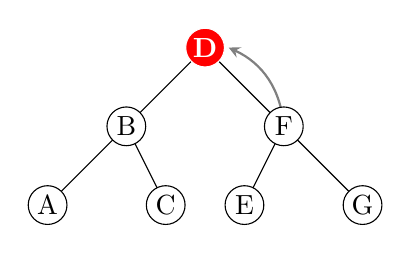
\begin{tikzpicture}[arrow/.style = {thick,-stealth}]
                \draw (0, 5) -- (-1,4);
                \draw (0, 5) -- (1,4);
                \draw (-1,4) -- (-2,3);
                \draw (-1,4) -- (-0.5,3);
                \draw (1,4) -- (2,3);
                \draw (1,4) -- (0.5,3);
                \draw[arrow,gray] (1,4) to[bend right] (0.3,5);
            
                \draw[white,fill=red] 
                    (0,5)  circle (7pt) node {\textbf{D}};
                \draw[fill=white] 
                    (-1,4) circle (7pt) node {B};
                \draw[fill=white] 
                    (1,4)  circle (7pt) node {F};
                \draw[fill=white] 
                    (-2,3) circle (7pt) node {A};
                \draw[fill=white] 
                    (-0.5,3) circle (7pt) node {C};
                \draw[fill=white] 
                    (0.5,3)  circle (7pt) node {E};
                \draw[fill=white] 
                    (2,3)  circle (7pt) node {G};
            \end{tikzpicture}
            \\  \footnotesize 
            11. Finished.
            \\  \footnotesize 
            Output: \texttt{D B A C F E G}
        \end{tabular} ~\\~\\

        Hopefully these steps help you better visualize the recursive
        nature of tree traversal.

    \newpage

        % -------------------------------------------------------------%
        % - QUESTION --------------------------------------------------%
        % -------------------------------------------------------------%
        \stepcounter{question}
        \begin{question}{\thequestion}{2}

            Traverse the following tree using \textbf{pre-order} traversal. Write
            out each Node as you ``process" it. ~\\
            
            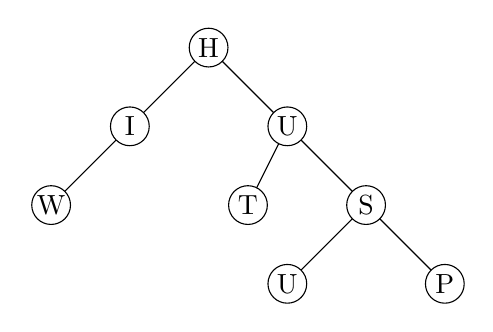
\begin{tikzpicture}
                \draw (0, 5) -- (-1,4);
                \draw (0, 5) -- (1,4);
                \draw (-1,4) -- (-2,3);
                \draw (1,4) -- (2,3);
                \draw (1,4) -- (0.5,3);
                \draw (2,3) -- (1,2);
                \draw (2,3) -- (3,2);
            
                \draw[fill=white] 
                    (0,5)  circle (7pt) node {H};
                \draw[fill=white] 
                    (-1,4) circle (7pt) node {I};
                \draw[fill=white] 
                    (-2,3) circle (7pt) node {W};
                \draw[fill=white] 
                    (1,4)  circle (7pt) node {U};
                \draw[fill=white] 
                    (0.5,3)  circle (7pt) node {T};
                \draw[fill=white] 
                    (2,3)  circle (7pt) node {S};
                \draw[fill=white] 
                    (1,2)  circle (7pt) node {U};
                \draw[fill=white] 
                    (3,2)  circle (7pt) node {P};
            \end{tikzpicture}

            \solution{
                H I W U T S U P
            }{ }
            
        \end{question}

        \hrulefill
        
        % -------------------------------------------------------------%
        % - QUESTION --------------------------------------------------%
        % -------------------------------------------------------------%
        \stepcounter{question}
        \begin{question}{\thequestion}{2}

            Traverse the following tree using \textbf{post-order} traversal. Write
            out each Node as you ``process" it. ~\\
            
            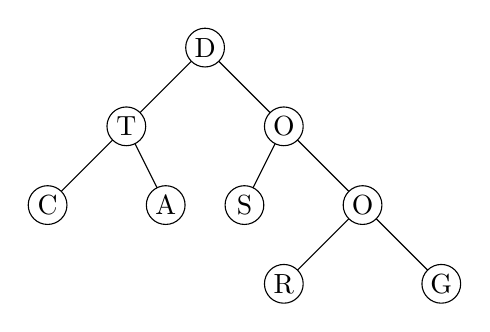
\begin{tikzpicture}
                \draw (0, 5) -- (-1,4);
                \draw (0, 5) -- (1,4);
                \draw (-1,4) -- (-2,3);
                \draw (-1,4) -- (-0.5,3);
                \draw (1,4) -- (2,3);
                \draw (1,4) -- (0.5,3);
                \draw (2,3) -- (1,2);
                \draw (2,3) -- (3,2);
            
                \draw[fill=white] 
                    (0,5)  circle (7pt) node {D};
                \draw[fill=white] 
                    (-1,4) circle (7pt) node {T};
                \draw[fill=white] 
                    (1,4)  circle (7pt) node {O};
                \draw[fill=white] 
                    (-2,3) circle (7pt) node {C};
                \draw[fill=white] 
                    (-0.5,3) circle (7pt) node {A};
                \draw[fill=white] 
                    (0.5,3)  circle (7pt) node {S};
                \draw[fill=white] 
                    (2,3)  circle (7pt) node {O};
                \draw[fill=white] 
                    (1,2)  circle (7pt) node {R};
                \draw[fill=white] 
                    (3,2)  circle (7pt) node {G};
            \end{tikzpicture}

            \solution{
                C A T S R G O O D
            }{  }
            
        \end{question}

        \hrulefill

        % -------------------------------------------------------------%
        % - QUESTION --------------------------------------------------%
        % -------------------------------------------------------------%
        \stepcounter{question}
        \begin{question}{\thequestion}{2}

            Traverse the following tree using \textbf{in-order} traversal. Write
            out each Node as you ``process" it. ~\\
            
            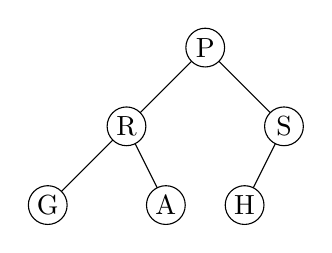
\begin{tikzpicture}
                \draw (0, 5) -- (-1,4);
                \draw (0, 5) -- (1,4);
                \draw (-1,4) -- (-2,3);
                \draw (-1,4) -- (-0.5,3);
                \draw (1,4) -- (0.5,3);
            
                \draw[fill=white] 
                    (0,5)  circle (7pt) node {P};
                \draw[fill=white] 
                    (-1,4) circle (7pt) node {R};
                \draw[fill=white] 
                    (1,4)  circle (7pt) node {S};
                \draw[fill=white] 
                    (-2,3) circle (7pt) node {G};
                \draw[fill=white] 
                    (-0.5,3) circle (7pt) node {A};
                \draw[fill=white] 
                    (0.5,3)  circle (7pt) node {H};
            \end{tikzpicture}
            
            \solution{
                G R A P H S
            }{  }
            
        \end{question}

        \newpage

        % -------------------------------------------------------------%
        % - QUESTION --------------------------------------------------%
        % -------------------------------------------------------------%
        \stepcounter{question}
        \begin{question}{\thequestion}{3}

            A \textbf{binary search tree} is a type of tree where each node
            can have 0, 1, or 2 children, but no more than 2.
            For any Node $n$, any nodes to the \textbf{left} of $n$ are less than $n$.
            Similarly, any nodes to the \textbf{right} of $n$ are greater than $n$.

            ~\\
            When the first node is added to a binary tree, it becomes the \textbf{root}.
            When subsequent nodes are added, we traverse the tree, moving to the left
            or right until we find an available space.

            ~\\
            For the following, there is a list of nodes in the order added to a tree.
            Draw out the binary tree once all nodes are added.

            \paragraph{Example:}
                Add: \texttt{C, B, D, A} ~\\
                
                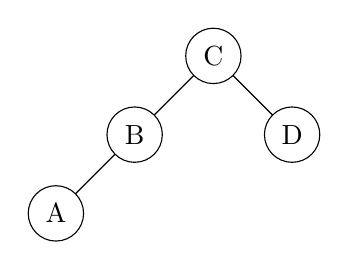
\begin{tikzpicture}
                    \draw (0,3) -- (-1,2) -- (-2,1);
                    \draw (0,3) -- (1,2);
                    
                    \filldraw[black,fill=white] (0,3) circle (10pt) node {C};
                    \filldraw[black,fill=white] (-1,2) circle (10pt) node {B};
                    \filldraw[black,fill=white] (1,2) circle (10pt) node {D};
                    \filldraw[black,fill=white] (-2,1) circle (10pt) node {A};
                \end{tikzpicture}

            \begin{itemize}
                \item[a.]   Add: \texttt{B, A, D, C, F, E}
                    \solution{}{ \vspace{3cm} }
                    
                \item[b.]   Add: \texttt{A, B, C, D, E}
                    \solution{}{ \vspace{3cm} }
                    
                \item[c.]   Add: \texttt{E, D, C, B, A}
                    \solution{}{ \vspace{3cm} }
                    
            \end{itemize}
        

            
        \end{question}

        \newpage


        % -------------------------------------------------------------%
        % - QUESTION --------------------------------------------------%
        % -------------------------------------------------------------%
        \stepcounter{question}
        \begin{question}{\thequestion}{1}
            
            For a \textbf{binary search tree}, we have a Node declared like this:
                    
\footnotesize 
\begin{verbatim}
template <typename T>
struct Node
{
    T data;
    Node* ptrLeft;
    Node* ptrRight;
};
\end{verbatim}
\normalsize

            And the following variables are already declared:

\begin{verbatim}
Node<char> nodeA;
Node<char> nodeB;
Node<char> nodeC;
Node<char> nodeD;
\end{verbatim}

            For each tree generated by adding nodes in the given order,
            write out the
            code (or pseudocode) to relate each node together. \\
            (e.g. \texttt{nodeA->ptrLeft = \&nodeB;})
            
            \begin{itemize}
                \item[a.]   \texttt{B, A, D, C}
                    \solution{}{ \vspace{3cm} }
                    
                \item[b.]   \texttt{A, B, C, D}
                    \solution{}{ \vspace{3cm} }

                \item[c.]   \texttt{D, C, B, A}
                    \solution{}{ \vspace{3cm} }
                    
            \end{itemize}
            
        \end{question}


    \newpage

    \subsection{Thinking in subtrees}

    WIP

    \newpage
    
    \subsection{Balanced trees}

    The same set of data can be arranged in a binary search tree
    in different ways, depending on the order that items are added to it.

    For example, lets add the numbers 1 through 7 to a binary tree
    in different orders.

    \begin{figure}[h]
        \begin{center}
            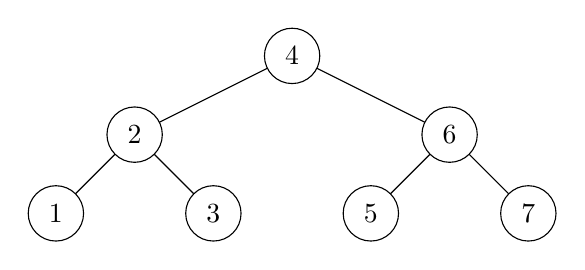
\begin{tikzpicture}
                \draw (0,3) -- (-2,2);
                \draw (-2,2) -- (-3,1);
                \draw (-2,2) -- (-1,1);
                \draw (0,3) -- (2,2);
                \draw (2,2) -- (1,1);
                \draw (2,2) -- (3,1);
                
                \filldraw[fill=white] (0, 3) circle (10pt) node {4};
                \filldraw[fill=white] (-2,2) circle (10pt) node {2};
                \filldraw[fill=white] (-3,1) circle (10pt) node {1};
                \filldraw[fill=white] (-1,1) circle (10pt) node {3};
                \filldraw[fill=white] (2,2) circle (10pt) node {6};
                \filldraw[fill=white] (1,1) circle (10pt) node {5};
                \filldraw[fill=white] (3,1) circle (10pt) node {7};
            \end{tikzpicture}
        \end{center}
        \caption{Add numbers: 4, 2, 1, 3, 6, 5, 7}
    \end{figure}

    Adding numbers like this gives us a nice binary search tree -
    it is not heavily skewed to one side or the other. This tree
    is actually \textbf{balanced}.

    \begin{quote}
        ``a binary tree is \textbf{height balanced}, or simply \textbf{balanced},
        if the height of any node's right subtree differs from the height of the node's
        left subtree by no more than 1.''
        
        \footnotesize
        From Data Abstraction \& Problem Solving with C++: Walls and Mirrors 7th ed, by Carrano and Henry, page 452
    \end{quote}

    However, if we add these numbers in an order such that each new number
    is greater than the last one, everything gets added to one side of the tree:

    \begin{figure}[h]
        \begin{center}
            \begin{tikzpicture}
                \draw (0,6) -- (1,5.5) -- (2,5) -- (3,4.5) -- (4,4) -- (5,3.5) -- (6,3);
                
                \filldraw[fill=white] (0, 6) circle (7pt) node {1};
                \filldraw[fill=white] (1, 5.5) circle (7pt) node {2};
                \filldraw[fill=white] (2, 5) circle (7pt) node {3};
                \filldraw[fill=white] (3, 4.5) circle (7pt) node {4};
                \filldraw[fill=white] (4, 4) circle (7pt) node {5};
                \filldraw[fill=white] (5, 3.5) circle (7pt) node {6};
                \filldraw[fill=white] (6, 3) circle (7pt) node {7};
            \end{tikzpicture}
        \end{center}
        \caption{Add numbers: 1, 2, 3, 4, 5, 6, 7}
    \end{figure}

    This binary tree is no more efficient to search from a sorted linear array,
    because everything is off to one side.

    \subsection{Full trees}

    \begin{quote}
        ``In a \textbf{full binary tree} of height $h$, all nodes that are at a level less than $h$
        have two children each.''
        
        \footnotesize
        From Data Abstraction \& Problem Solving with C++: Walls and Mirrors 7th ed, by Carrano and Henry, page 451
    \end{quote}
    
    
    \subsection{Complete trees}
    
    \begin{quote}
        ``A \textbf{complete binary tree} of height $h$ is a binary tree that is full down to level $h-1$, with level $h$
        filled in from left to right. [...]

        More formally, a binary tree $T$ of height $h$ is complete if

        \begin{enumerate}
            \item   All nodes at level $h-2$ and above have two children each, and
            \item   When a node at level $h-1$ has children, all nodes to its left at the same level have two children each, and
            \item   When a node at level $h-1$ has one child, it is a left child
        \end{enumerate}

        [...] Note that a full binary tree is complete.''
        
        \footnotesize
        From Data Abstraction \& Problem Solving with C++: Walls and Mirrors 7th ed, by Carrano and Henry, page 451
    \end{quote}
    
\end{document}









